\section*{\nr.1 \titone (25 Punkte)}
\begin{enumerate}[(a)]
\item 
Wir sind davon ausgegangen, dass zum Zeitpunkt $t=0$ der Stromkreis geschlossen wurde, mathematisch durch die Heaviside-Funktion ausgedrückt:
\begin{equation}
Q(t) = Q_0 e^{-\gamma t} e^{i\omega_0 t}\Theta(t); \quad \gamma\in\mathbb{R}_{>0}
\end{equation}
Dadurch muss in der Fouriertransformation das Integral nur für positive Zeiten ausgewertet werden. Es folgt für die Fourier-Transformierte:
\begin{align}
q(\omega) &= \frac{1}{\sqrt{2\pi}}\int_0^{\infty} e^{-\gamma t} e^{i\omega_0 t} e^{-i\omega t} \,\mathrm{d}t\\ 
&= \frac{Q_0}{\sqrt{2\pi}} \left. \frac{1}{-\gamma-i(\omega-\omega_0)}e^{[-\gamma-i(\omega-\omega_0)]t} \right|_{t=0}^{\infty} \\
\intertext{Wegen $\gamma>0$ verschwindet die obere Grenze und es folgt:}
q(\omega)&= \frac{Q_0}{\sqrt{2\pi}} \frac{1}{\gamma-i(\omega+\omega_0)}
\end{align}
\item Zur Berechnung des Spektrums wird zunächst das komplex Konjugierte zu $q(\omega)$ berechnet:
\begin{equation}
q^*(\omega) =\frac{Q_0}{\sqrt{2\pi}} \left[ \frac{\gamma-i(\omega-\omega_0)}{\gamma^2+(\omega-\omega_0)^2}\right]^* = \frac{Q_0}{\sqrt{2\pi}} \frac{\gamma+i(\omega-\omega_0)}{\gamma^2+(\omega-\omega_0)^2}
\end{equation}
Für das Spektrum folgt dann direkt:
\begin{equation}
|q(\omega)|^2 = q(\omega) * [q(\omega)]^* = \frac{Q_0^2}{2\pi} \frac{1}{\gamma^2+(\omega-\omega_0)^2}
\end{equation}
\item Die Phase $\phi(\omega)$ ergibt sich durch:
\begin{equation}
\tan \varphi(\omega) = \frac{\text{Im}(q)}{\text{Re}(q)} = \frac{\omega_0-\omega}{\gamma}
\end{equation}
Also folgt:
\begin{equation}
\varphi(\omega) = \arctan \frac{\omega_0-\omega}{\gamma}
\end{equation}

\item
Eine Abbildung des Spektrums ist durch \vref{fig:spektrum} für verschiedene $\gamma$ gegeben. Man erkennt, dass die Breite des Spektrums sich mit zunehmendem $\gamma$ relativ zu seiner (gleichzeitig sinkenden) Höhe vergrößert. Die Phase ist in \vref{fig:phase} abgebildet.
\begin{figure}[htbp]
\centering
% GNUPLOT: LaTeX picture with Postscript
\begingroup
  \makeatletter
  \providecommand\color[2][]{%
    \GenericError{(gnuplot) \space\space\space\@spaces}{%
      Package color not loaded in conjunction with
      terminal option `colourtext'%
    }{See the gnuplot documentation for explanation.%
    }{Either use 'blacktext' in gnuplot or load the package
      color.sty in LaTeX.}%
    \renewcommand\color[2][]{}%
  }%
  \providecommand\includegraphics[2][]{%
    \GenericError{(gnuplot) \space\space\space\@spaces}{%
      Package graphicx or graphics not loaded%
    }{See the gnuplot documentation for explanation.%
    }{The gnuplot epslatex terminal needs graphicx.sty or graphics.sty.}%
    \renewcommand\includegraphics[2][]{}%
  }%
  \providecommand\rotatebox[2]{#2}%
  \@ifundefined{ifGPcolor}{%
    \newif\ifGPcolor
    \GPcolortrue
  }{}%
  \@ifundefined{ifGPblacktext}{%
    \newif\ifGPblacktext
    \GPblacktextfalse
  }{}%
  % define a \g@addto@macro without @ in the name:
  \let\gplgaddtomacro\g@addto@macro
  % define empty templates for all commands taking text:
  \gdef\gplbacktext{}%
  \gdef\gplfronttext{}%
  \makeatother
  \ifGPblacktext
    % no textcolor at all
    \def\colorrgb#1{}%
    \def\colorgray#1{}%
  \else
    % gray or color?
    \ifGPcolor
      \def\colorrgb#1{\color[rgb]{#1}}%
      \def\colorgray#1{\color[gray]{#1}}%
      \expandafter\def\csname LTw\endcsname{\color{white}}%
      \expandafter\def\csname LTb\endcsname{\color{black}}%
      \expandafter\def\csname LTa\endcsname{\color{black}}%
      \expandafter\def\csname LT0\endcsname{\color[rgb]{1,0,0}}%
      \expandafter\def\csname LT1\endcsname{\color[rgb]{0,1,0}}%
      \expandafter\def\csname LT2\endcsname{\color[rgb]{0,0,1}}%
      \expandafter\def\csname LT3\endcsname{\color[rgb]{1,0,1}}%
      \expandafter\def\csname LT4\endcsname{\color[rgb]{0,1,1}}%
      \expandafter\def\csname LT5\endcsname{\color[rgb]{1,1,0}}%
      \expandafter\def\csname LT6\endcsname{\color[rgb]{0,0,0}}%
      \expandafter\def\csname LT7\endcsname{\color[rgb]{1,0.3,0}}%
      \expandafter\def\csname LT8\endcsname{\color[rgb]{0.5,0.5,0.5}}%
    \else
      % gray
      \def\colorrgb#1{\color{black}}%
      \def\colorgray#1{\color[gray]{#1}}%
      \expandafter\def\csname LTw\endcsname{\color{white}}%
      \expandafter\def\csname LTb\endcsname{\color{black}}%
      \expandafter\def\csname LTa\endcsname{\color{black}}%
      \expandafter\def\csname LT0\endcsname{\color{black}}%
      \expandafter\def\csname LT1\endcsname{\color{black}}%
      \expandafter\def\csname LT2\endcsname{\color{black}}%
      \expandafter\def\csname LT3\endcsname{\color{black}}%
      \expandafter\def\csname LT4\endcsname{\color{black}}%
      \expandafter\def\csname LT5\endcsname{\color{black}}%
      \expandafter\def\csname LT6\endcsname{\color{black}}%
      \expandafter\def\csname LT7\endcsname{\color{black}}%
      \expandafter\def\csname LT8\endcsname{\color{black}}%
    \fi
  \fi
    \setlength{\unitlength}{0.0500bp}%
    \ifx\gptboxheight\undefined%
      \newlength{\gptboxheight}%
      \newlength{\gptboxwidth}%
      \newsavebox{\gptboxtext}%
    \fi%
    \setlength{\fboxrule}{0.5pt}%
    \setlength{\fboxsep}{1pt}%
\begin{picture}(7936.00,5102.00)%
    \gplgaddtomacro\gplbacktext{%
      \csname LTb\endcsname%
      \put(550,704){\makebox(0,0)[r]{\strut{}$0$}}%
      \put(682,484){\makebox(0,0){\strut{}$0$}}%
      \put(4042,461){\makebox(0,0)[l]{\strut{}$\omega_0$}}%
    }%
    \gplgaddtomacro\gplfronttext{%
      \csname LTb\endcsname%
      \put(176,2770){\rotatebox{-270}{\makebox(0,0){\strut{}$|q(\omega)|^2$}}}%
      \put(4110,154){\makebox(0,0){\strut{}$\omega$}}%
      \csname LTb\endcsname%
      \put(6552,4664){\makebox(0,0)[r]{\strut{}$\gamma=\num{0.8}$}}%
      \csname LTb\endcsname%
      \put(6552,4444){\makebox(0,0)[r]{\strut{}$\gamma=\num{1,0}$}}%
      \csname LTb\endcsname%
      \put(6552,4224){\makebox(0,0)[r]{\strut{}$\gamma=\num{1.2}$}}%
      \csname LTb\endcsname%
      \put(6552,4004){\makebox(0,0)[r]{\strut{}$\gamma=\num{1.4}$}}%
    }%
    \gplgaddtomacro\gplbacktext{%
      \csname LTb\endcsname%
      \put(550,704){\makebox(0,0)[r]{\strut{}$0$}}%
      \put(682,484){\makebox(0,0){\strut{}$0$}}%
      \put(4042,461){\makebox(0,0)[l]{\strut{}$\omega_0$}}%
    }%
    \gplgaddtomacro\gplfronttext{%
      \csname LTb\endcsname%
      \put(176,2770){\rotatebox{-270}{\makebox(0,0){\strut{}$|q(\omega)|^2$}}}%
      \put(4110,154){\makebox(0,0){\strut{}$\omega$}}%
      \csname LTb\endcsname%
      \put(6552,4664){\makebox(0,0)[r]{\strut{}$\gamma=\num{0.8}$}}%
      \csname LTb\endcsname%
      \put(6552,4444){\makebox(0,0)[r]{\strut{}$\gamma=\num{1,0}$}}%
      \csname LTb\endcsname%
      \put(6552,4224){\makebox(0,0)[r]{\strut{}$\gamma=\num{1.2}$}}%
      \csname LTb\endcsname%
      \put(6552,4004){\makebox(0,0)[r]{\strut{}$\gamma=\num{1.4}$}}%
    }%
    \gplbacktext
    \put(0,0){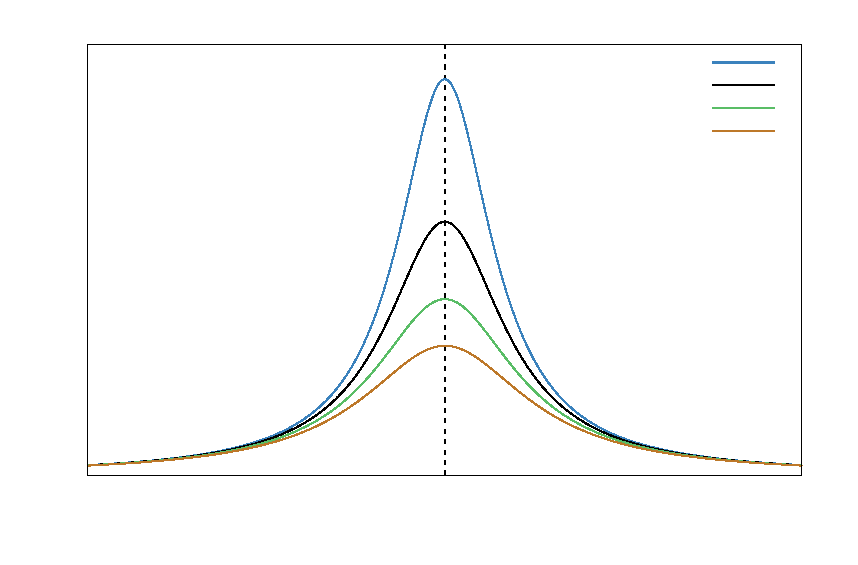
\includegraphics{spektrum}}%
    \gplfronttext
  \end{picture}%
\endgroup

\caption{Spektrum $q(\omega)$ in \emph{einheitenlosen} Größen. Die relative Breite des Spektrums wächst mit steigendem $\gamma$.}
\label{fig:spektrum}
\end{figure}

\begin{figure}[htbp]
\centering
% GNUPLOT: LaTeX picture with Postscript
\begingroup
  \makeatletter
  \providecommand\color[2][]{%
    \GenericError{(gnuplot) \space\space\space\@spaces}{%
      Package color not loaded in conjunction with
      terminal option `colourtext'%
    }{See the gnuplot documentation for explanation.%
    }{Either use 'blacktext' in gnuplot or load the package
      color.sty in LaTeX.}%
    \renewcommand\color[2][]{}%
  }%
  \providecommand\includegraphics[2][]{%
    \GenericError{(gnuplot) \space\space\space\@spaces}{%
      Package graphicx or graphics not loaded%
    }{See the gnuplot documentation for explanation.%
    }{The gnuplot epslatex terminal needs graphicx.sty or graphics.sty.}%
    \renewcommand\includegraphics[2][]{}%
  }%
  \providecommand\rotatebox[2]{#2}%
  \@ifundefined{ifGPcolor}{%
    \newif\ifGPcolor
    \GPcolortrue
  }{}%
  \@ifundefined{ifGPblacktext}{%
    \newif\ifGPblacktext
    \GPblacktextfalse
  }{}%
  % define a \g@addto@macro without @ in the name:
  \let\gplgaddtomacro\g@addto@macro
  % define empty templates for all commands taking text:
  \gdef\gplbacktext{}%
  \gdef\gplfronttext{}%
  \makeatother
  \ifGPblacktext
    % no textcolor at all
    \def\colorrgb#1{}%
    \def\colorgray#1{}%
  \else
    % gray or color?
    \ifGPcolor
      \def\colorrgb#1{\color[rgb]{#1}}%
      \def\colorgray#1{\color[gray]{#1}}%
      \expandafter\def\csname LTw\endcsname{\color{white}}%
      \expandafter\def\csname LTb\endcsname{\color{black}}%
      \expandafter\def\csname LTa\endcsname{\color{black}}%
      \expandafter\def\csname LT0\endcsname{\color[rgb]{1,0,0}}%
      \expandafter\def\csname LT1\endcsname{\color[rgb]{0,1,0}}%
      \expandafter\def\csname LT2\endcsname{\color[rgb]{0,0,1}}%
      \expandafter\def\csname LT3\endcsname{\color[rgb]{1,0,1}}%
      \expandafter\def\csname LT4\endcsname{\color[rgb]{0,1,1}}%
      \expandafter\def\csname LT5\endcsname{\color[rgb]{1,1,0}}%
      \expandafter\def\csname LT6\endcsname{\color[rgb]{0,0,0}}%
      \expandafter\def\csname LT7\endcsname{\color[rgb]{1,0.3,0}}%
      \expandafter\def\csname LT8\endcsname{\color[rgb]{0.5,0.5,0.5}}%
    \else
      % gray
      \def\colorrgb#1{\color{black}}%
      \def\colorgray#1{\color[gray]{#1}}%
      \expandafter\def\csname LTw\endcsname{\color{white}}%
      \expandafter\def\csname LTb\endcsname{\color{black}}%
      \expandafter\def\csname LTa\endcsname{\color{black}}%
      \expandafter\def\csname LT0\endcsname{\color{black}}%
      \expandafter\def\csname LT1\endcsname{\color{black}}%
      \expandafter\def\csname LT2\endcsname{\color{black}}%
      \expandafter\def\csname LT3\endcsname{\color{black}}%
      \expandafter\def\csname LT4\endcsname{\color{black}}%
      \expandafter\def\csname LT5\endcsname{\color{black}}%
      \expandafter\def\csname LT6\endcsname{\color{black}}%
      \expandafter\def\csname LT7\endcsname{\color{black}}%
      \expandafter\def\csname LT8\endcsname{\color{black}}%
    \fi
  \fi
    \setlength{\unitlength}{0.0500bp}%
    \ifx\gptboxheight\undefined%
      \newlength{\gptboxheight}%
      \newlength{\gptboxwidth}%
      \newsavebox{\gptboxtext}%
    \fi%
    \setlength{\fboxrule}{0.5pt}%
    \setlength{\fboxsep}{1pt}%
\begin{picture}(7936.00,5102.00)%
    \gplgaddtomacro\gplbacktext{%
      \csname LTb\endcsname%
      \put(550,2771){\makebox(0,0)[r]{\strut{}$0$}}%
      \put(682,484){\makebox(0,0){\strut{}$0$}}%
      \put(4042,469){\makebox(0,0)[l]{\strut{}$\omega_0$}}%
    }%
    \gplgaddtomacro\gplfronttext{%
      \csname LTb\endcsname%
      \put(176,2770){\rotatebox{-270}{\makebox(0,0){\strut{}$\varphi(\omega)$}}}%
      \put(4110,154){\makebox(0,0){\strut{}$\omega$}}%
      \csname LTb\endcsname%
      \put(6552,4664){\makebox(0,0)[r]{\strut{}$\gamma=\num{0.8}$}}%
      \csname LTb\endcsname%
      \put(6552,4444){\makebox(0,0)[r]{\strut{}$\gamma=\num{1,0}$}}%
      \csname LTb\endcsname%
      \put(6552,4224){\makebox(0,0)[r]{\strut{}$\gamma=\num{1.2}$}}%
      \csname LTb\endcsname%
      \put(6552,4004){\makebox(0,0)[r]{\strut{}$\gamma=\num{1.4}$}}%
    }%
    \gplgaddtomacro\gplbacktext{%
      \csname LTb\endcsname%
      \put(550,2771){\makebox(0,0)[r]{\strut{}$0$}}%
      \put(682,484){\makebox(0,0){\strut{}$0$}}%
      \put(4042,469){\makebox(0,0)[l]{\strut{}$\omega_0$}}%
    }%
    \gplgaddtomacro\gplfronttext{%
      \csname LTb\endcsname%
      \put(176,2770){\rotatebox{-270}{\makebox(0,0){\strut{}$\varphi(\omega)$}}}%
      \put(4110,154){\makebox(0,0){\strut{}$\omega$}}%
      \csname LTb\endcsname%
      \put(6552,4664){\makebox(0,0)[r]{\strut{}$\gamma=\num{0.8}$}}%
      \csname LTb\endcsname%
      \put(6552,4444){\makebox(0,0)[r]{\strut{}$\gamma=\num{1,0}$}}%
      \csname LTb\endcsname%
      \put(6552,4224){\makebox(0,0)[r]{\strut{}$\gamma=\num{1.2}$}}%
      \csname LTb\endcsname%
      \put(6552,4004){\makebox(0,0)[r]{\strut{}$\gamma=\num{1.4}$}}%
    }%
    \gplbacktext
    \put(0,0){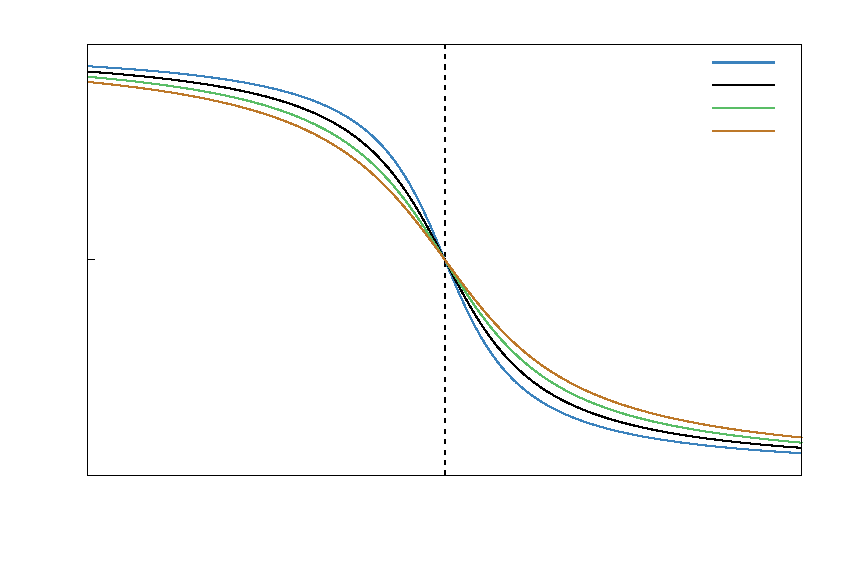
\includegraphics{phase}}%
    \gplfronttext
  \end{picture}%
\endgroup

\caption{Phase $\varphi(\omega)$ in \emph{einheitenlosen} Größen}
\label{fig:phase}
\end{figure}




\end{enumerate}